% =================================
%      Particle Accelerators
% =================================
\section{\review{Particle Accelerators}}

% Too much history for Ewen :(
%
%Particle accelerators are a relatively recent development, driven by the particle physics
%field~\cite{bryant_brief_1994}. The first accelerators, at the beginning of the 20th century, were
%able to accelerate particles up to energies of a few MeV using electric fields.
%
%The Cockcroft Walton generator was powerful enough to split an atom for the first time in
%1932~\cite{poole_cockcrofts_2007}, less than 100 years ago. Its design used capacitors and diodes
%to double the voltage at each stage, with its main limitation being the breakdown voltage of the
%capacitors. The Van de Graaff generator, created around the same time, was able to accelerate
%particles up to tens of MeV. They are still in use today~\cite{lebois_rapport_2020} due to their
%capability of producing a wide variety of ion beams with energies ranging from hundreds of KeV to
%hundreds of MeV in the \textit{Tandem} form~\cite{hinterberger_electrostatic_2006}.
%
%Radiofrequency generators with alternating electric fields and drift tubes, first created by 
%Rolf Wideröe in the late 1920s, mark the beginning of modern accelerator
%technology~\cite{vretenar_radio_2011}. Rapidly evolving, particle accelerators progressed from
%accelerating particles to a few keV in linear accelerators to now TeV in circular accelerators,
%called synchrotrons.
%
%While single-beam synchrotrons can be used for fixed-target experiments, only a fraction of the
%energy is available on impact. Dual-beam machines were more suitable for high energy physics
%experiments. The first hadron collider, the ISR, was built at CERN in 1971 with an energy
%of 62 GeV, taking its beam from the Proton Synchrotron (PS)~\cite{philip_cerns_2011}. 
%
%Particle accelerators are still rapidly evolving. Several have been built in the past, and several
%are now either under construction or in the design study phase. New acceleration and focusing
%techniques are being developed, making the machines smaller. It is an exciting time for all fields
%that might benefit from energetic particles, whether in fundamental research, medical, industrial or
%security applications.

% ================================

Particle accelerators have come a long way since their invention in the 20th century, when they
could only reach a few MeV of energy using electric fields~\cite{bryant_brief_1994}. Today, they
achieve much higher energies, up to the TeV range, allowing for more detailed investigations into
particle physics.

One of the major milestones in accelerator development was the shift to circular accelerators, known
as synchrotrons. By the 1970s, machines like the ISR at CERN could accelerate particles to 62 GeV
using beams from the Proton Synchrotron (PS)~\cite{philip_cerns_2011}, enabling significant advances
in particle physics experiments.

As accelerators have evolved, so has the need for better control of particle beams. Managing beam
stability and lifetime has become crucial, especially in modern machines like the LHC. 

Considerable advancements have been made in both radiofrequency acceleration technologies,
collimation, superconducting magnets and beam dynamics to keep beams stables and on track, even at
high energies. These improvements are not only important for physics research but are also used in
medical and industrial fields.

In modern accelerators, precise beam control is necessary to ensure efficient and accurate
collisions. Correcting beam optics has moved from being just a theoretical exercise to an essential
part of operations. This has led to a shift away from empirical methods, where trial and error were
common, towards more direct, quantitative approaches that provide a detailed and accurate correction
of beam dynamics. These advancements not only improve performance but also play a key role in
designing future accelerators with better stability and efficiency.


% --------------------------------
%          CERN Complex
% --------------------------------
\subsection{\review{The CERN Complex}}

CERN is a large laboratory located on the border of France and Switzerland, near Geneva. Although
well-known for discoveries in particle physics, studies are also conducted on medical applications,
biology, radiation hardness or material science.
Several accelerators are part of the accelerator complex, as illustrated in
\cref{fig:introduction:cern_complex}. A large number of fixed target experiments exist, whose
beams are delivered by various accelerators depending on their needs. These experiments are often
renewed~\footnote{Up to date information can be found on
\href{https://home.cern/science/experiments}{https://home.cern/science/experiments}.}.

The largest part of the CERN accelerator complex is the LHC. The LINAC4, PSB, PS and SPS
accelerators serve as pre-injectors to the LHC.

\begin{figure}[!htb]
    \centering
    \includegraphics[width=1\textwidth]{images/cern_complex.png}
    \caption{Schematic illustration of the accelerator complex at CERN. Most accelerators are both
    used as injectors for the LHC or to provide beams to fixed target
    experiments~\cite{noauthor_cern_2022}.}
    \label{fig:introduction:cern_complex}
\end{figure}


% --------------------------------
%              LHC
% --------------------------------
\subsection{\review{The Large Hadron Collider}}

The Large Hadron Collider (LHC) is a circular particle accelerator primarily designed to collide
protons for fundamental particle physics research. It can also occasionally collide ions such as
oxygen or lead for specific studies. At the time of writing, in 2024, it holds several records,
such as being the largest and most powerful accelerator in the world, at nearly 27 km long. The LHC
is composed of two beam pipes, capable of accelerate two particle beams from an injection energy
of $450$ GeV to an energy of $6,800$ GeV, before colliding them in four detectors: ATLAS, CMS, Alice
and LCHb.

Well-publicized, the LHC is often depicted via its superconducting dipole magnets, housed in blue
cryostats, aimed at cooling the coils. \Cref{fig:3d_cut_dipole} shows a 3D cut of such magnets. The
LHC is mostly composed of these \textit{main} dipoles, holding $1,232$ of them, each about 14 meters
long. 
Particles in the LHC travel at nearly the speed of light ($99.99999905\%$), completing roughly
$11,200$ turns around the tunnel each second. To generate the intense magnetic fields needed to
deflect such high-momentum particles, currents of approximately $12,000$ amperes are supplied to the
magnets.  However, conventional materials like copper would overheat and melt under this current
load, necessitating the use of superconducting materials such as niobium-titanium (NbTi).


\begin{figure}[!htb]
    \centering
    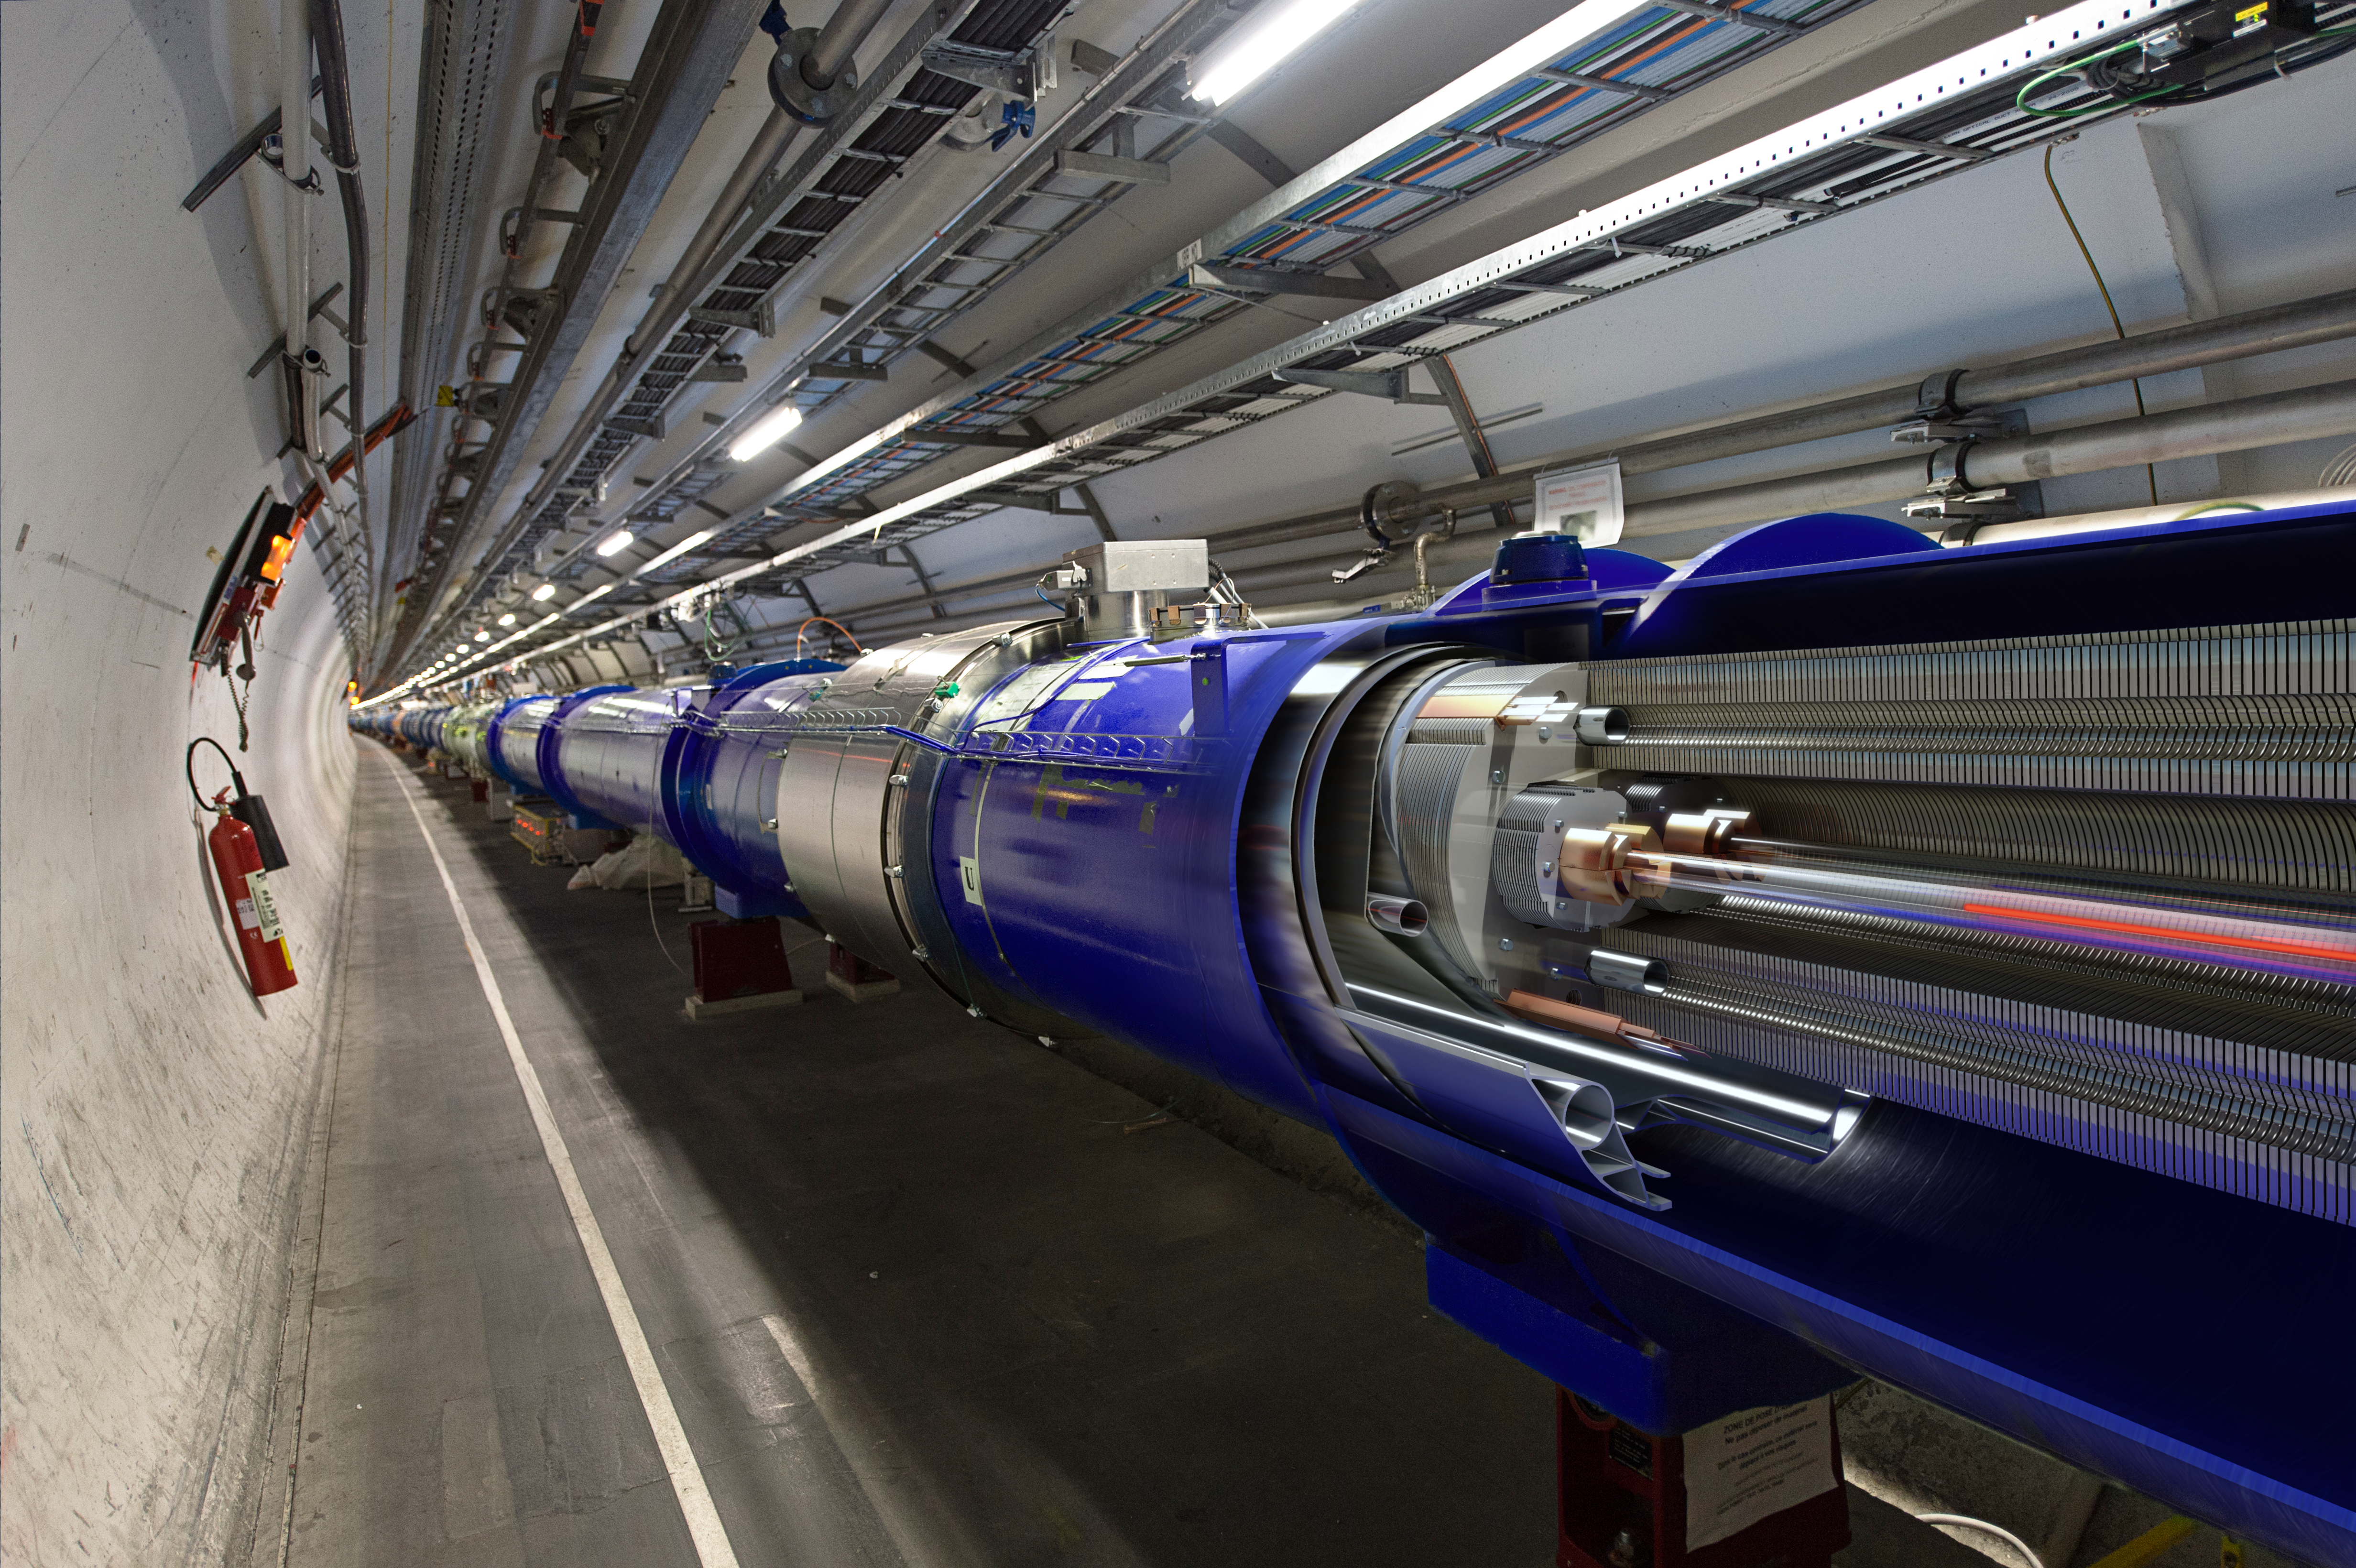
\includegraphics[width=0.8\textwidth]{chapters/01_Introduction/images/lhc_3D_cut.png}
    \caption{3D cut of a main LHC dipole~\cite{noauthor_cern_nodate}. Both beam pipes can be seen
    surrounded by the coils, strongly clamped by the yokes.}
    \label{fig:3d_cut_dipole}
\end{figure}


% -------------------------------
%   Straight Sections and Arcs
\subsubsection{\mread{Straight Sections and Arcs}}

The LHC is not a perfect circle. It is indeed composed of eight \textit{straight} sections, called
the \textit{Insertion Regions} (IRs) where detectors or specific instrumentation are placed.
Connecting those sections, the \textit{arcs} are where the majority of the magnets and their
correctors are located, along with some instrumentation like beam position monitors.
\Cref{fig:introduction:lhc_irs} shows the arcs as well as the purpose of each straight section.

\begin{figure}[!htb]
    \centering
    \includegraphics[width=0.5\textwidth]{./images/irs.png}
    \caption{Schematic of the LHC layout.}
    \label{fig:introduction:lhc_irs}
\end{figure}


% -------------------------------
%          Arc Cells
\subsubsection{\mread{Arc Cells}}

Each arc is made up of 23 cells. Magnets are organized in a standard FODO structure
(see \cref{section:courant_snyder}), as shown in \cref{fig:introduction:lhc_arc_cell}.
\textit{Dipoles} are responsible for bending the trajectory of the particles. Their associated
correctors, the orbit correctors, mitigate any possible drift in the path.
\textit{Quadrupoles} are used to control the beam size along the ring. Their effect is focusing in
one plane and defocusing in the other. Their associated correctors control the frequency of
oscillations of the beam (see tune, \cref{section:courant_snyder}) and possible field imperfections.
\textit{Sextupoles} correct chromaticity, a misfocus from quadrupoles due to particles having
a different momentum than the reference particle.
\textit{Octupoles} are used to stabilize the beam by introducing Landau
Damping~\cite{gareyte_landau_1997}. The associated correctors correct higher-order chromaticity
effects as well as amplitude-dependant tune shifts.
\textit{Decapoles} correctors aim at correcting an even higher chromaticity order.

\begin{figure}[H]
    \centering
    \includegraphics[width=1\textwidth]{./images/lhc_cell.png}
    \caption{Schematic of an LHC Arc cell~\cite{bruning_lhc_2004}.}
    \label{fig:introduction:lhc_arc_cell}
\end{figure}



% -------------------------------
%            Cycles
\subsubsection{\mread{Cycles}}

During the operation of the LHC, the machine goes through several states, each defined for specific 
scenarios~\cite{wenniger_lhc_2019}.

A common example is the operational cycle of the LHC, illustrated in \cref{fig:cern_complex:cycle}.
Initially, the magnets are pre-cycled~\cite{bottura_pre-cycles_2010} without any beam circulating,
to ensure a reproducible magnetic state. Their current is then increased to accept particles at the
injection energy of 450 GeV. To verify the machine's proper functioning, a probe bunch of reduced
intensity is first injected, at around $10^{10}$ particles. The number of bunches and their
intensity are then gradually increased to obtain the desired scheme needed for collisions, which
varies throughout the year based on experimental demands. The number of bunches and their intensity
can be adjusted as needed to ensure the machine's safety. A common scheme in 2024 is to inject about
2350 bunches, with around $1.5 \cdot 10^{11}$ particles in each bunch, for collisions. Optics
measurements, due to their destructive nature, typically use between one and three \textit{pilot}
bunches at a lower intensity of $10^{10}$ particles.

The current in the magnets is then increased along with adjustments in the phase and voltage of the
RF system to accelerate the particles to an energy of 6.8 TeV. During this ramp, the beam is
initially squeezed at the Interaction Points. However, further squeezing is limited by the
detectors' resolution, which is insufficient to accurately reconstruct a large number of collision
events simultaneously. Collisions then start, while levelling the $\beta^*$ at the ATLAS and CMS
experiments relative to the remaining beam intensity, ensuring optimal performance of the detectors.

\begin{figure}[!htb]
    \includegraphics[width=\textwidth]{./images/lhc_cycle.pdf}
    \caption{Simplified illustration of a standard LHC cycle. Adapted
    from~\cite{felix_soubelet_local_2023}.}
    \label{fig:cern_complex:cycle}
\end{figure}
